\documentclass[11pt]{article}

\usepackage{xeCJK}
\usepackage{graphicx}
\usepackage{amsmath}
\usepackage{booktabs}
\usepackage{cite}
\usepackage{float}
\usepackage{indentfirst}

\setCJKmainfont[BoldFont=SourceHanSerifSC-Bold]{SourceHanSerifSC-Regular}
\setCJKsansfont[BoldFont=SourceHanSansSC-Bold]{SourceHanSansSC-Regular}
\setCJKmonofont{STFangsong}
\setlength{\parindent}{2em}

\renewcommand{\baselinestretch}{1.5}

\usepackage{xcolor}
\usepackage{listings}

\definecolor{mGreen}{rgb}{0,0.6,0}
\definecolor{mGray}{rgb}{0.5,0.5,0.5}
\definecolor{mPurple}{rgb}{0.58,0,0.82}
\definecolor{backgroundColour}{rgb}{0.95,0.95,0.92}

\lstdefinestyle{CStyle}{
    backgroundcolor=\color{backgroundColour},   
    commentstyle=\color{mGreen},
    keywordstyle=\color{magenta},
    numberstyle=\tiny\color{mGray},
    stringstyle=\color{mPurple},
    basicstyle=\footnotesize,
    breakatwhitespace=false,         
    breaklines=true,                 
    captionpos=b,                    
    keepspaces=true,                 
    numbers=left,                    
    numbersep=5pt,                  
    showspaces=false,                
    showstringspaces=false,
    showtabs=false,                  
    tabsize=2,
    language=C
}

\title{OSH可行性报告\\[2ex]文件多路传输系统}
\author{徐直前 PB16001828\\吴永基 PB16001676\\黄子昂 PB16001840\\金朔苇 PB16001696\\}
\date{\today}
\begin{document}

\maketitle
\tableofcontents

\section{项目简介}
\section{项目背景}
通常在软件开发中使用的多人协作解决方案,就是Git这种版本控制系统了。
Git这种版本控制系统通常是每个用户各自工作,完成自己的部分代码,
最后再将自己的代码merge到项目中去。在此过程中,客户端不需要和服务器以及其他客户端进行通许。
所以,这里也就不需要一个锁的机制,用户就可以做到并发地编辑。
但是在实时协作系统中同步性就成为了最大的问题了。同步性

让我们来看一个例子。假设客户端Alice、Bob和服务器端开始的状态都是ABCD

现在Alice要在D(即第四个字符(假设offset从0开始,D的offset为3))
之前插入字符X,同时Bob要删除字符B,那么由于延时的问题,那么Alice可能会认为插入在删除之前执行,
但是服务器认为删除操作是在插入操作之前执行的。那么Alice看到的结果就是ACXD,而服务器上的结果是ACDX。
这显然就出现来致命的问题,每个编辑者看到的结果不一样。显然,需要一个精心设计的机制才能解决这个问题。

我们在调研报告中已经调研过Google Docs,Apple iWork,Microsoft Office Online、石墨文档,
还有像EtherPad、Firepad这样的开源项目。其中我们并没有发现能同时较好的保证一致性、实现历史版本、的产品。
并且大多都是富文本编辑器,而现在的很多技术人员和产品经理都大多都偏好Markdown这样的写作方式,
但几乎没有能支持Markdown编辑的文档协作产品,更没有任何产品能对每个用户进行精细的权限控制,
而不是笼统的只能对整篇文档设置只读或者可编辑。


\section{理论依据}
\subsection{编辑锁}
编辑锁是最简单的实现方式,每
个人在编辑文件的同时,对文件进行上锁,
其他所有用户都不能编辑此文件,这样的实现最大的好处就是逻辑简单,
而且完全避免了冲突。然而,这种方式的效率很低,
类似于计算机网络中对同一链路复用的时候使用了纯ALOHA协议,
在负载较高的情况下,冲突几率很高,排队时间时间长,应用在多人协作编辑时,
可能会出现这样的极端情况:某人几乎长时间占用编辑权限,导致其他人一直处于冲突的状态而无法编辑。
我们可以参考计算机网络中的CSMA协议,可以大大提高复用效率,并且减少冲突。对于大流量端淹没小流量端的问题,
我们可以借鉴滑动窗口协议,使每个用户都有可以忍受的服务质量。然而,由于延迟和时序等原因,
如果要恢复由冲突导致失效的指令,单纯的编辑锁是没办法实现的。如果这些失效的指令丢失了,
就会导致修改状态不稳定,或是呈现的编辑结果与修改结果不符,这也是用户很难接受的。

\subsection{GNU diff-patch}
相比于编辑锁,该算法解决了冲突带来的糟糕体验,
并且有许多早期的协作编辑软件都是基于这种方法实现的。假设两台终端合作编辑一份文件,
每台终端连接至服务器后,获取该文件的一个副本,然后在本地对副本进行编辑,
每隔一段时间或者等用户停止编辑一段时间后,将编辑后的文件副本上传给服务器,
服务器对新旧版本进行diff运算,并且智能合并。之后,将更改的patch广播给每个用户来进行同步。
该算法有一个明显的缺陷:GNU diff通过行匹配,在两个用户同时编辑同一行后,智能合并就失效了,
出现无法避免的冲突。在负载较高的情况下,上行与下传会占用大量I/O资源,并且智能合并的结果也更加不可预测。

该方法的实时性不够强,但这也成为了一种优势,即对于延迟的要求低,而且通过适当的预测算法,只上传一部分进行diff,缓解带宽压力。
另外一个优势是,可以方便人工核对,然后进行选择合并。

\subsection{Myer's diff-patch}
在GNU diff-patch算法中,
我们提到diff是行为单位进行检测并合并的,
但仍然无法避免高几率发生的冲突,而且在智能合并的复杂度与随着负载的增加而极大增加,
结果的不可预测性提高。Myer对此方案进行了改进,将检测的粒度降低为字,使得冲突的几率和合并结果的随机性和波动性减小。
冲突虽然不可能完全避免,但只会在对同一个字编辑的时候发生,这时可能会丢失字符。
对于普通文本来说,这是可以忍受的情况。对于包含代码等对正确性要求极高的富文本文件,修复丢失的字符会占用大量的资源。


\subsection{Operational Transformation}
\subsubsection{简介}
Operational Transformation 则是一种相对较为先进的解决方案,
能较好的解决同步性问题。这项技术相对来说也是较为复杂,
已经在学术界和工业界被研究了二十多年了。著名的Apache Wave和Google Docs的核心技术便是Operational Transformation。

Operational Transformation
最早是在1989年由C. Ellis and S. Gibbs提出的。
但是过了几年,就有人发现了原始的方案拥有一些正确性的问题,
也提出了不同的解决方案。随后十几年,无数研究者又对OT进行了不断的扩充和升级。

OT这项技术,顾名思义就是当文档的状态发生变化时,
就对用户发送的操作请求进行变化,从而保证每个用户文档状态的同步。
在OT中,用户的所有编辑都会被转变成一个操作(operation)。
当两个操作被应用到一篇文档时,我们会根据第一个操作对文档的改变,
计算第二个操作该如何变化,以保证第二个操作的一正常进行,
保留第一个操作原本对文档的操作意图。

\subsubsection{核心思想}
我们把这个协作系统中的每个参与者叫作一个站点(site),
通常一个站点就对应一个用户的工作站。当然,也有一些机器会对应多个站点。我们在这里假设每个站点都可以和其他站点之间相互通信。

这里,我们来定义一下这个协作系统的结构$G=<S, O>$这里$S$是站点的集合,$O$是操作(operators)的集合。

每一个站点都由一个站点进程(site process),
一个站点对象(site object),以及一个唯一的站点标识符(site identifier)构成。
其中站点对象就是我们需要尽力维护站点对象的一致性,使得每个用户看到的结果尽可能一样。
一个站点对象的结构是由应用程序决定的。 操作的集合O也取决于站点对象,比如一个文本编辑系统的站点对象可能就包含一个字符串,
并且定义操作集合O={O1, O2}。
\begin{center}
O1 = insert[X; P]   在位置P插入字符X\\
O2 = delete[P]	    删除位置P的字符
\end{center}

例如之前的例子「ABCD」。

比如说现在一个用户想在D之前插入字符X,那么他就需要发送操作O1[X; 3]。

站点进程需要处理三种问题:
\begin{enumerate}
    \item 操作的生成:将用户的编辑转换成操作,并且向整个网络中的其他站点广播
    \item 操作的接受:从其他站点接受操作请求
    \item 操作的执行:执行一个操作请求
\end{enumerate}

回到ABCD这个例子中
\begin{enumerate}
    \item Alice发送了操作O1[X; 3]插入X,Bob发送了操作O2[1]删除B
    \item 服务器首先接到了Bob的请求,删除了B,现在文本变为了ACD
    \item 服务器接受了Alice的操作O1[X; 3],但是现在正确插入的位置应该变为了2,服务器会自动完成这一操作的变化
    \item 现在Alice、Bob和服务器都认为文档的状态是ACXD了,这样就保证了一致性。
\end{enumerate}

在这样一个协作系统中,我们需要一个服务器来保存文档的「真理」。这样即使一个客户端下线了,我们同样可以从服务器上获取文档。

一般来说,我们有如下两种操作:
\begin{itemize}
    \item 包含变换(Inclusion Transformation):用IT(a, b)表示,对操作a进行变换,以将操作b的影响包含在内
    \item 排除变换(Exclusion Transformation):用ET(a, b)表示,对操作a进行变换,以将操作b的影响排除在外
\end{itemize}

现在让我们来看IT变换的一个例子:
假设我们要对两个插入操作Insert[p1, c1], Insert[p2, c2]
进行IT变换(插入的均是单个字母,p1,p2 为插入位置,c1, c2为插入字符。
那么我们的变换函数将是这样实现的:

\begin{lstlisting}[style=CStyle]
IT_INS_INS (Insert[p2, c2], Insert[p1, c1]) {
    if ((p2 < p1) || (p1 == p2 && u2 > u1))	return Insert[p2, c2];
    else return Insert[p2 + 1, c2];
}
\end{lstlisting}
以上代码用user identifier来标示用户操作的优先级。

\begin{figure}[H]
    \begin{center}
    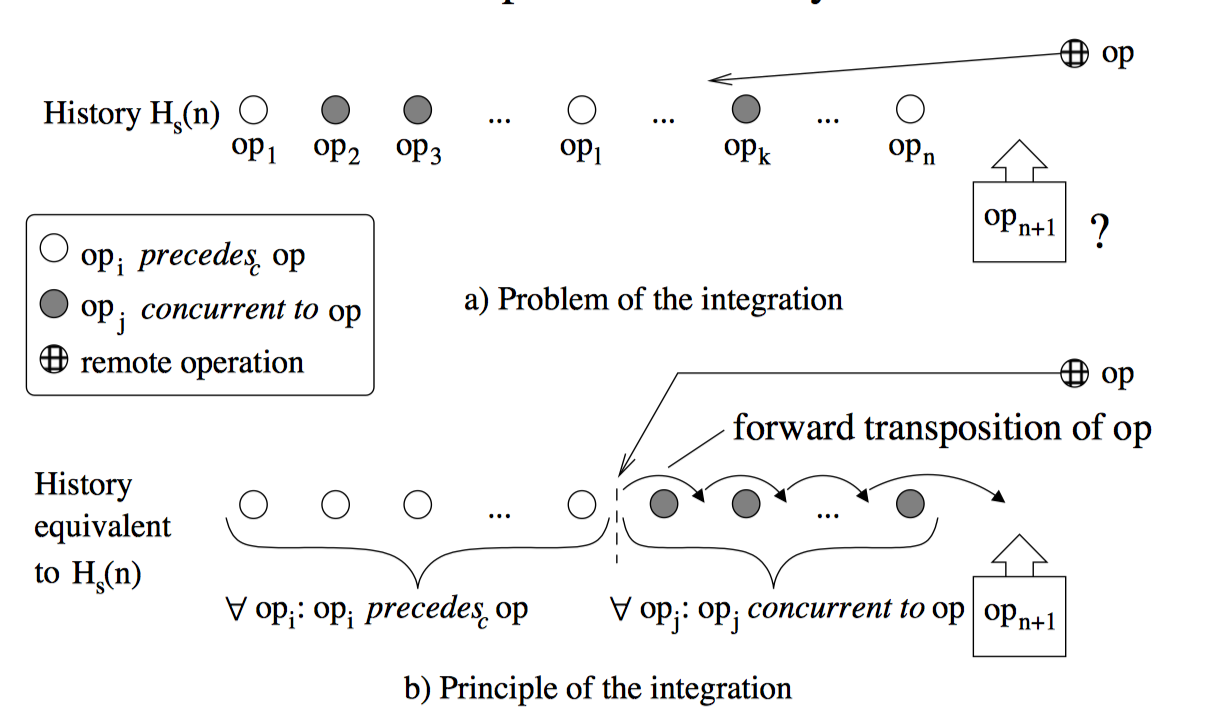
\includegraphics[width=0.8\textwidth]{figures/ot_transformation.png}
    \caption{操作变换}
    \end{center}
\end{figure}

相比于以上character-wise的,实现string-wise的操作算法就会复杂多了,因为
\begin{itemize}
    \item 字符串的删除会覆盖一个范围
    \item 并发的字符串删除可能会产生重叠(overlap)
    \item 之前插入操作可能会被之后的插入和删除操作改变
\end{itemize}
OT中最大的一个难题就是实现撤销的操作了。
在OT中我们要撤销操作O,那么我们就要消除操作O的一切影响,
同时保留其他所有操作的影响。在一个单用户文本编辑器中,这一点很容易实现,
因为操作都是线性的。但在多用户协作系统中,这就成为了一个难题,操作变成非线性的了。
\subsubsection{不同算法比较}
\paragraph{dOPT算法}
没有中心服务器,且会遇到dOPT-puzzle的问题,这个算法并不正确。
\begin{figure}[H]
    \begin{center}
    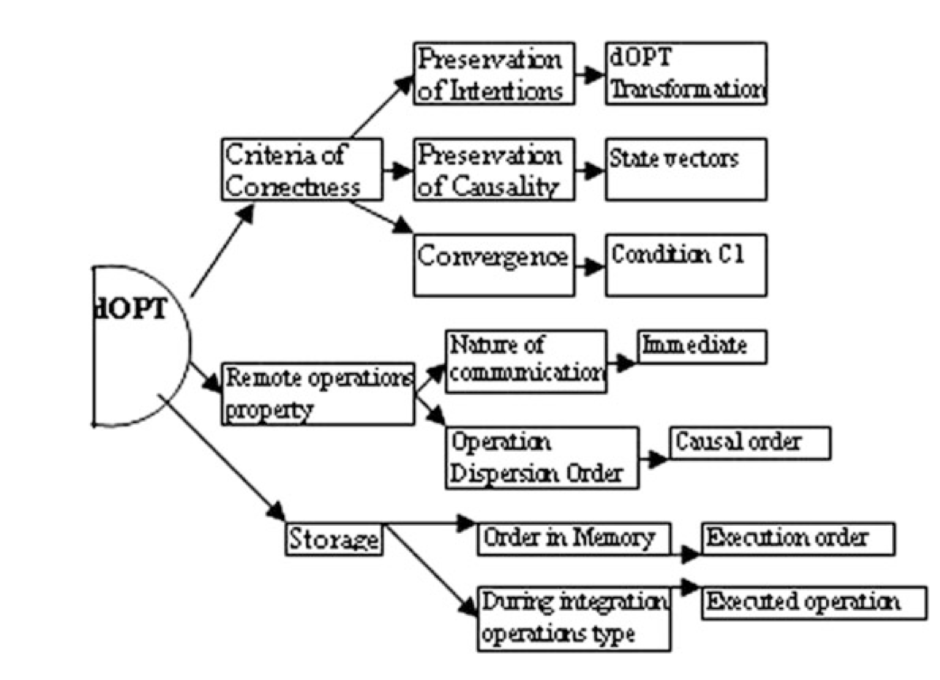
\includegraphics[width=0.67\textwidth]{figures/dOPT.png}
    \caption{dOPT}
    \end{center}
\end{figure}
\paragraph{adOPTed算法}
dOPT算法的改进
\begin{figure}[H]
    \begin{center}
    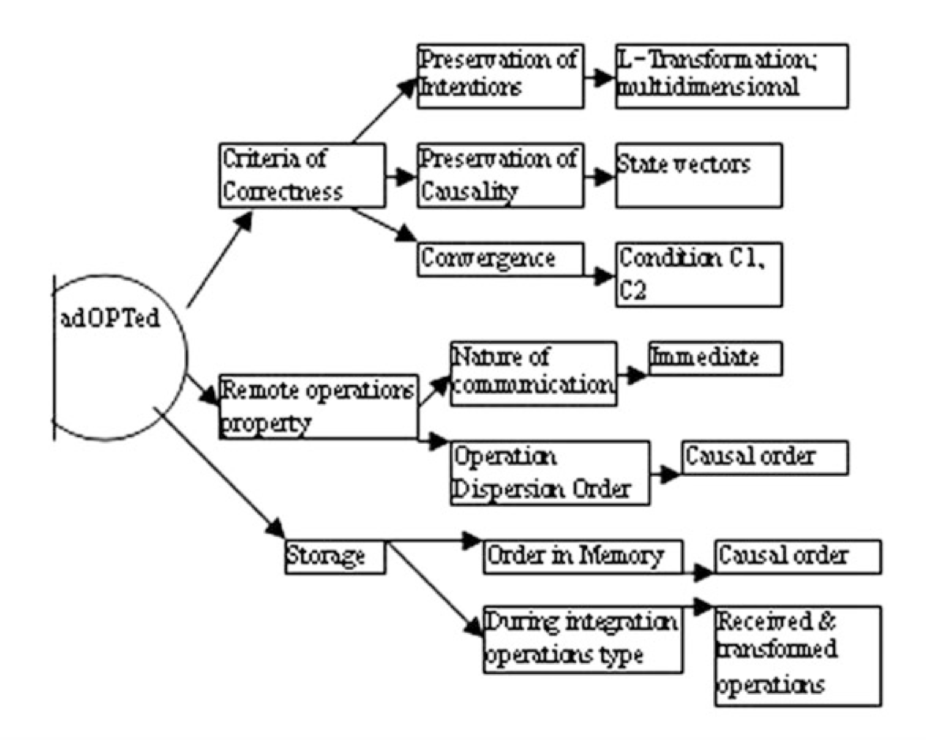
\includegraphics[width=0.67\textwidth]{figures/adOPTed.png}
    \caption{adOPTed}
    \end{center}
\end{figure}
\paragraph{GOT算法}
GOT算法很好的实现了一直行,并且支持undo/do/redo。但是它只能支持两种基本字符串操作:插入/删除。
\begin{figure}[H]
    \begin{center}
    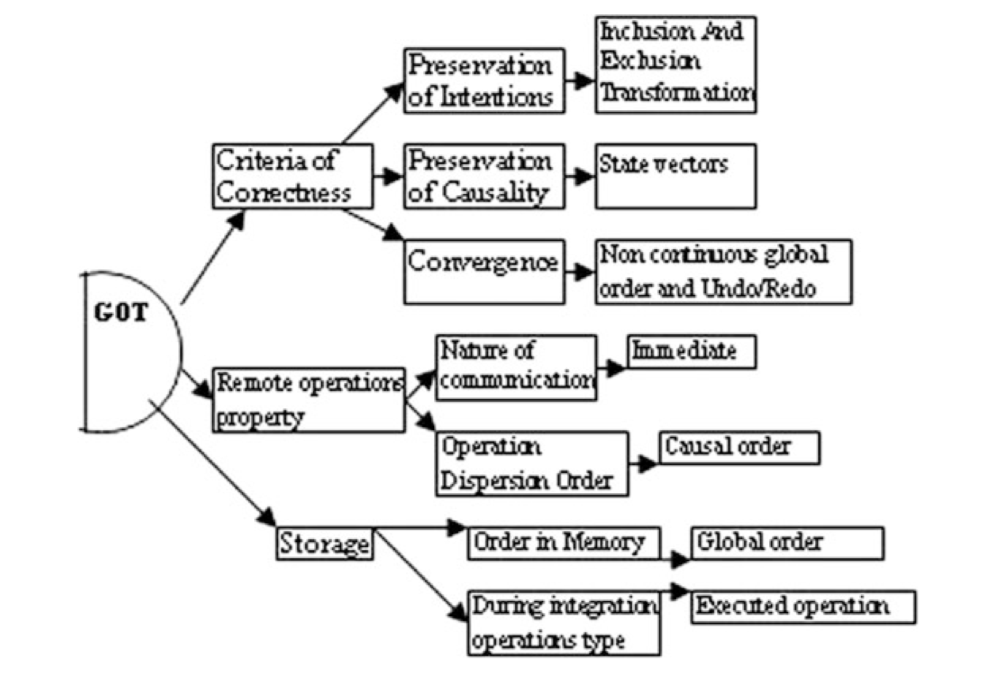
\includegraphics[width=0.67\textwidth]{figures/GOT.png}
    \caption{GOT}
    \end{center}
\end{figure}
\subsection{CRDT}
\subsubsection{简介}
CRDT是Convergent and Commutative Replicated Data Type 
的缩写,换言之“无冲突可复制型数据”。

人类目前实际可行的构建超大规模系统的比较好的解决方案就是利用分布式文件系统。但是分布式文件系统正确性很难保证
CAP定理证明了在构建分布式系统的时候,Consistency(一致性),
Availability(可用性),Partition tolerance(分区容错性),
这三者只可以同时选择两样。分区容错性是实际运营的分布式系统所必需的。
所以必须在一致性和可用性中选择其一。
选择一致性,构建的就是强一致性系统,比如符合ACID特性的数据库系统。选择可用性,
构建的就是最终一致性系统。前者的特点是数据落地即是一致的,但是可用性不能时时保证,
这意思就是,有时系统在忙着保证一致性,无法对外界服务。后者的特点是时时刻刻都保证可用性,
用户随时都可以访问,但是各个节点之间会存在不一致的时刻。最终一致性的系统不是不保证一致性,
而是不在保证可用性和分区容错性的同时保证一致性。最终还是要在最终一致性的各节点之间处理数据,使他们达到一致。

CRDT是一个解决这种问题的很好的方案。
其思想从总体上来说就是利用多存储的信息来在某一时刻解决一致性问题。
在实际系统中应用,我们必须要考虑很多的数据类型和应用场景。
CRDT就是这样一些适应于不同场景的可以保持最终一致性的数据结构的统称。
举例来说,假如我们想利用分布式系统来解决一个账户的支出收入问题。
假设这个账户是T,初始化有100块钱,用户可以通过系统里面好几个节点,
例如A,B,C,访问它。那么我们最终的分布式系统,都会给A,B,C三者权限以对账户进行操作。
这时我们就需要多加入一些信息来保证信息的正确性。此时我们这样设计这样的一个系统,
每个系统存储的不是一个最终的数值,而是一系列包含了时刻与余额的记录,
假设我们的系统从t0时刻开始的,那么在我们的例子里面,t1时刻
\begin{enumerate}
    \item A系统存储的是(t0,100), (t1,110)
    \item B系统存储的是(t0,100), (t1,90)
    \item C系统存储的是(t0,100), (t1,100)
\end{enumerate}
这样的结构使得我们在传输了足够的信息之后,都能达成一致性。
例如对于C系统,当收到足够多的信息,即是除自己之外所有的节点信息(A和B)后,就得到了这样的结论
\begin{enumerate}
    \item A系统在t0至t1之间产生的变化是+10
    \item B系统在t0至t1之间产生的变化是-10
    \item C系统在t0至t1之间产生的变化是+0
    \item A和B系统与C在t0时数据一致,在t1之后未至t2之前一致的数据应为100+10-10+0=100
\end{enumerate}
类似的,在A和B上也可以这样判断

CRDT不是一个基于共识的系统,
其使用一些简单的数学性质来确保事件的连续性。
CRDT快速将备份整合为和使用序列处理效果相同的通用的状态。
由于CRDT不需要同步,一个升级会被快速地处理,并不被网络的延迟性所影响。

\subsubsection{概念}
\paragraph{原子和对象}
一个进程可以存储原子和对象。一个原子是一个基本的不可被改变的数据类型,
原子是由它的字面意思被识别;如果他们有相同的内容,那么原子可以被认为是相同的。
原子的类型在这篇文章中被划分为整数,字符串,集合,元组,和他们的不可改变的操作。原子的类型可以被写成更低级的形式比如集合。

一个对象是可改变的,重复的数据类型。
对象的种类是被大写化的。例如”Set”。
一个对象拥有一个身份,可能是任意对象的一个内容,
一个初始状态,并且一个由操作构成的界面。
两个操作拥有相同的身份但是却定位在不同的进程中,这样的情况被称为另一个的复制品。

\paragraph{操作}
该环境由未指定的客户端组成,
这些客户端通过调用其接口中的操作来查询和修改对象状态,
并针对他们选择的称为源副本的副本进行查询和修改。查询在本地执行,即完全在一个副本上执行。
更新有两个阶段:第一,客户端在源处调用操作,该操作可能会执行一些初始处理。然后,更新将异步传输到所有副本;这是下游部分。
\section{技术依据}
\section{创新点}

\nocite{*}
\bibliographystyle{plain}
\bibliography{ref}
\end{document}